
\section{CMS Pixel Detector Phase 1 Upgrade project}
\label{sec:upgrade}

%%% The paragraph below is just a starter that Alice contributed.
%%% It is used partially in the final text.

% The CMS collaboration plans to upgrade the CMS pixel detector to
% include a four-layer barrel and three endcap disks (on each end) with
% improved data acquisition throughput. As the LHC luminosity increases
% with more underlying events captured per beam crossing, the present
% electronics readout system would incur significant dead time. A new
% digital pixel readout chip (ROC) is being produced so that instead of
% the 40 MHz analog readout, there will be a 400 Mbps digital
% readout. This necessitates a re-design of the electronics downstream
% from the silicon pixel modules. The upgraded detector also includes a
% super light-weight mechanical design with CO2 cooling which will
% significantly reduce the materials in the detector for better tracking
% and vertexing performance. The full detector is expected to be
% inserted in the CMS detector sometime in the 2017-2018 time
% period. The CMS upgrade plan is described in \cite{UpgradeProposal}.

% Possibly the new TDR can be quoted as well.

%--------------------
%\vspace{1cm}

%%% THE TEXT BELOW IS MOVED TO THE INTRO SECTION
% At the heart of CMS is the silicon pixel detector that provides three
% high-precision space point measurements to reconstruct charged
% particle trajectories. These three points are sufficient to produce
% good track information for the High Level Trigger (HLT) and for the
% efficient seeding of track reconstruction in the full tracker
% volume. The close proximity of the first detector layer to the
% interaction point (4.4 cm) minimizes multiple scattering effects and
% extrapolation uncertainties making the pixel information crucial for
% the reconstruction of the initial position and direction of the
% charged tracks. The pixel detector therefore plays a key role in the
% identification of primary vertices, secondary vertices, and secondary
% tracks. These elements are essential for the efficient identification
% of long-lived particles, such as b quarks, and for the search for new
% physics at the LHC.

%%% The paragraph below is from Daniela
%%% It has been changed and merged with the paragraph from Alice
% The present CMS pixel detector was conceived over 10 years ago and
% designed for a maximum luminosity of $1 \times 10^{34}$ cm$^{-2}$
% s$^{-1}$ and 25 ns bunch crossing. The LHC is now expected to exceed
% this peak luminosity already before the long shutdown 2 and perhaps to
% operate at 50 ns to maximize the integrated luminosity. The present
% pixel system will not be able to sustain the efficient operation in
% that condition due to large data losses in the read out chip (ROC) and
% must be replaced during or before long shutdown 2. The modular design
% of CMS allows good access to the pixel system, which can be easily
% extracted. In long shutdown 1 CMS plans to perform activities, such as
% replacing the current beam pipe, that facilitate the pixel replacement
% in a technical stop, if the replacement is ready and the LHC operating
% conditions require it.



The present CMS pixel detector was conceived over 10 years ago and
designed for a maximum luminosity of $1 \times 10^{34}$ cm$^{-2}$
s$^{-1}$ and 25 ns bunch crossing. The LHC is now expected to exceed
this peak luminosity already before the long shutdown 2 and perhaps to
operate at 50 ns to maximize the integrated luminosity. The present
pixel system will not be able to sustain the efficient operation in
that condition due to large data losses in the ROC.
The CMS collaboration plans to upgrade the pixel detector to include a
larger number of layers with a more optimal geometry, a new digital
ROC, and a redesigned data acquisition electronics downstream from the
silicon pixel modules. The new pixel detector will be significantly
more light-weight, which will lead to reduced distortion of particle
trajectories as they traverse the material of the detector. 

\begin{figure}[htb]
  \centering
  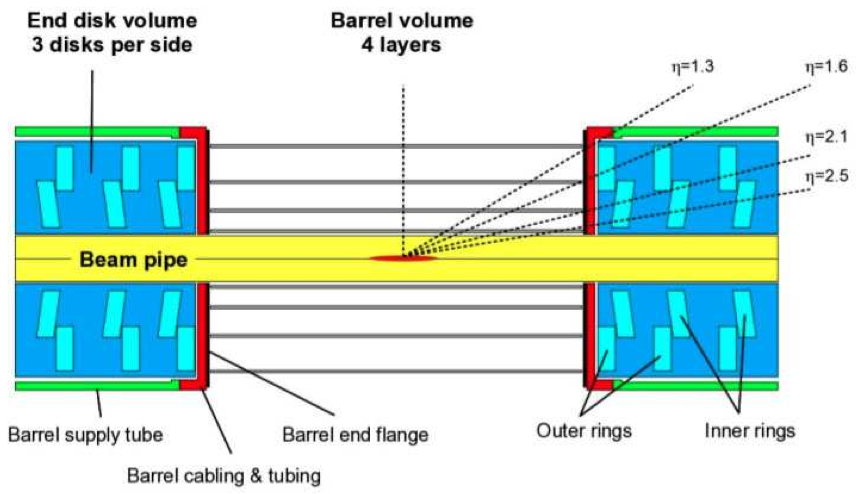
\includegraphics[width=0.7\textwidth]{Phase_1_pixel_detector.png}
  \caption{\label{fig:phase1pixels}
    Conceptual layout for the Phase 1 upgrade pixel detector.
  }
\end{figure}

The Phase~1 CMS pixel detector will have 4 barrel layers and 3 disks
in each endcap (Fig.~\ref{fig:phase1pixels}). The four barrel layers
are of equal length and are placed at radii of 3.9, 6.8, 10.9, and
16.0 cm. The three end-cap disks are placed on each side of the
central barrel detector, with a radial coverage from 4.5 cm to 16.1
cm.  The location of the disks along the beam line, with respect to
the interaction point, is 29.1~cm, 39.6~cm, and 51.6~cm. In the new
design, there will be only one type of module with 16 ROCs in a
$2\times 8$ arrangement. The digital readout of the new ROC will
operate at 400~Mbps instead of the present system's 40~MHz analog
readout. The 16-ROC modules will be mounted on ultra-lightweight
support structures integrated with the cooling distribution
system. Two-phase CO$_2$ cooling will replace the current single phase
C$_6$F$_{14}$ resulting in significant material reduction. Thin-walled
stainless steel pipes of 1.6~mm in diameter will be used to provide
enough cooling power for each pixel sub-assembly based on a continuous
loop. Further material reduction will be achieved by using longer
twisted pair or light-weight flex-cables to carry the signals to the
optical hybrid boards; these boards, as well as the port cards and
cooling manifolds, will be moved out of tracking region. The outer and
inner parts of the detector will be designed to allow the inner layers
and rings to be easily replaced after radiation damage.

%%% Commebted out, a bit too much detail
% For FPIX, this requires each half-disk be divided into an
% inner and outer ring.  Similar to the current detector, the blades in
% the forward disks are rotated by 20 degrees in a turbine like geometry
% to induce charge sharing. The separation of each half disk into an
% inner and outer assembly allows us to optimize the orientation and
% tilting to obtain the best position resolution in both radial and
% $\phi$ directions. Our baseline is to tilt the inner assemblies into
% an inverted cone at 12 degrees towards the interaction point.

%%% Again, this is good, but maybe a bit too much detail
% The upgraded pixel detector is constrained by the existing insertion
% volume and services. The upgraded detector must use the existing power
% cables, fibers, and cooling lines from the cooling plant. Cables,
% fibers, and other required utilities are already installed for 3
% forward disks; however, space for making changes to utilities is
% severely limited. The existing rail system for insertion and
% extraction will be used.  To improve the physics performance of a
% pixel detector in terms of impact parameter resolution and vertex
% resolution the first active layer should be as close as possible to
% the beam, requiring a new beam pipe of minimum radius consistent with
% the LHC aperture requirements.


The implementation of the Phase1 pixel detector would improve all aspects of CMS tracking:
\begin{itemize}
\item The addition of the extra layers will dramatically improve the
  efficiency and resolution of pixel-only tracks that are a crucial
  part of the High Level Trigger. Since the pixels are also used to seed full tracks
  this will increase the tracking efficiency and decrease the fake
  rate.
\item The decrease in the amount of material and the increase in the
  number of measurement points will improve the resolution of all
  track parameters.
\item The efficiency and resolution enhancements will lead to improved
  primary and secondary vertexing. Vertex reconstruction is essential
  to associate the final state particles with the correct primary
  vertex in the high pile-up environment. Secondary vertexing plays a
  key role in b-tagging and the search for various long-lived exotic
  states. The improvements in tracking efficiency, fake rate, impact
  parameter resolution, and vertexing contribute to significant
  improvements in the b-tagging performance of the tracker.
  Considering a luminosity of $2 \times 10^{34}$ cm$^{-2}$ s$^{-1}$
  with 25 ns bunch spacing, the upgraded detector would reduce the
  light quark background by a factor of 6 for a b-efficiency of 60\%,
  or conversely, it would increase the b-quark efficiency by
  approximately 50\% at the fixed light-quark efficiency of $5\times
  10^{-2}$.
\end{itemize}

\noindent
The improved performance of the CMS tracking system will in turn
significantly enhance the capability of the CMS experiment to pursue
its key physics goals, including investigation of the Electroweak
Symmetry Breaking mechanisms as well as the search for signs of
physics beyond the Standard Model.

The finalizing of the design of the Phase~1 pixel detector, its
construction, and commissioning into an integral part of the CMS
detector involves a significant amount of work. Many Universities from
the U.S., Europe, and other parts of the world, contribute to this
project. As for the present CMS pixel detector, the institutions
submitting this proposal are among the leaders within the US CMS
community on the R\&D, construction, and commissioning of the Phase~1
Forward Pixel Detector, while the Swiss institutions ETHZ, PSI, and
University of Zurich lead the Phase~1 Barrel Pixel Detector project.
Thus, the Phase~1 upgrade continues and deepens the collaboration between
the Swiss and U.S. Universities outlined in Section~\ref{sec:ties}.
An already mentioned important feature of the new design of the pixel
detector is the fact that both the Forward and the Barrel parts will
use exactly the same 16-ROC modules with exactly the same readout.
This provides for cooperation and trading experience in module
construction, testing, commissioning, and calibration, the topics
closely related to this proposal, as will be discussed in
Section~\ref{sec:projects}.


The modular design of CMS allows good access to the pixel system,
which can be easily extracted, thus the replacement can happen during
a technical stop (several month long) or a long shutdown of the LHC.
The new Phase~1 pixel detector is expected to be inserted in the CMS
detector sometime in the 2017-2018 time period. In more detail, the
CMS Phase~1 pixel detector upgrade plan is described in
\cite{UpgradeProposal}.

